\chapter{Detailed analysis of the state-of-art} \label{cpt:state-of-art}

This chapter will present a detailed analysis of the state-of-the-art in epileptic seizure prediction.

\section{Epileptic Seizure Detection and Prediction Techniques}
This section is not focused only on seizure prediction techniques. Instead seizure detection and prediction researches are analyzed as a whole, for various reasons \cite{gadhoumi_seizure_2016, bou_assi_towards_2017, natu_review_2022}:

\begin{itemize}
    \item lack of researches and publications strictly on seizure prediction 
    \item higher difficulty in separating preictal \gls{EEG} signals from interictal ones
    \item techniques that are more efficient in seizure detection generally grant good results for seizure prediction aswell
\end{itemize}

With these premises in mind, what follows is an overview of the best methods and techniques for seizure detection and prediction.

First of all it is important to remember that the success of a system is dependent on the statistical parameters and classification methods that it employs; choosing the appropriate parameters or features and classification methods is a significant challenge.

In time different approaches for seizure detection and prediction have been used, going from traditional feature extractions and analysis methods along with traditional machine learning algorithms for classification, to the most recent researches involving deep learning algorithms, as shown in Fig. \ref{fig:seizure-prediction-evolution-flow}.

\begin{figure}[ht]
    \centering
    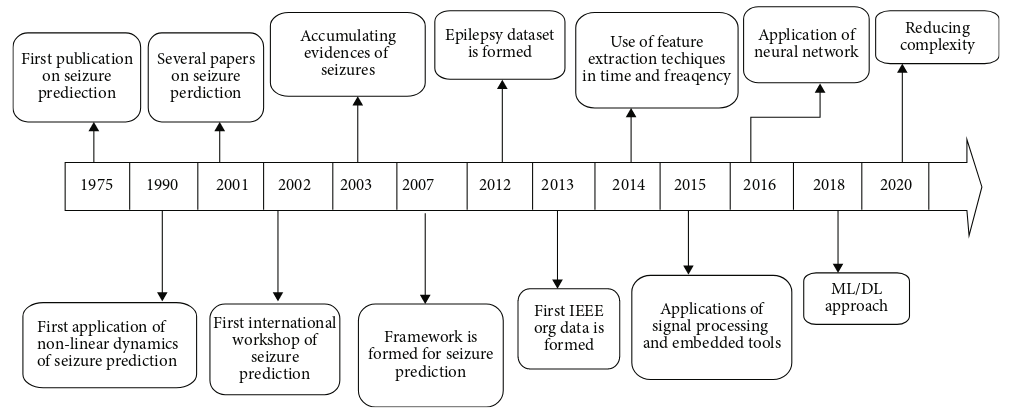
\includegraphics[width=1.0\textwidth]{images/State-of-art/seizure-prediction-evolution-flow.png}
    \caption{Seizure prediction and detection technologies - evolution flow \cite{natu_review_2022}}
    \label{fig:seizure-prediction-evolution-flow}
\end{figure}

\subsection{Traditional analysis methods and feature extraction}
During the 1970s, \gls{EEG} analysis involved the interpretation of \gls{EEG} waveforms using subjective and intuitive methods \cite{callaway_coupling_1974}. Over time, a variety of techniques have been developed to analyze subtle changes in the \gls{EEG} signal and have often been used for epileptic seizure detection and prediction \cite{natu_review_2022}. These methods can be broadly classified into four categories: time domain analysis, frequency domain analysis, time-frequency domain analysis, and nonlinear methods \cite{acharya_automated_2013}.

Depending on how many channels are involved in each feature extraction method, they can be distinguished in:
\begin{itemize}
    \item univariate, which sees the method applied independently on each channels
    \item bivariate, which sees the method applied on couple of channels
\end{itemize}

\begin{figure}[ht]
    \centering
    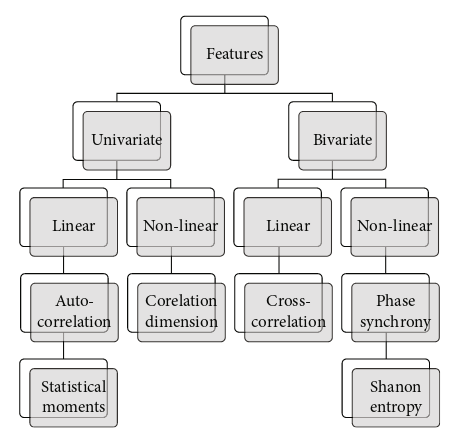
\includegraphics[width=0.75\textwidth]{images/State-of-art/univariate-bivariate-feature-extraction.png}
    \caption{Classification of some feature extraction methods based on the number of channels involved during said extraction \cite{natu_review_2022}}
    \label{fig:univariate-bivariate-feature-extraction}
\end{figure}

\subsubsection{Time domain methods}
Time domain analysis methods are used to study the \gls{EEG} signal in the time domain, rather than the frequency domain. These methods include linear prediction and component analysis \cite{acharya_automated_2013}. 

Linear prediction involves using a linear system to predict the output based on input and previous outputs.

Component analysis is an unsupervised method that maps data to a feature set, and it can be performed using principal component analysis, independent component analysis, or linear discriminant analysis. 
\gls{PCA} reduces high-dimensional data to a lower-dimensional orthogonal feature subspace, while \gls{ICA} decomposes multidimensional data into independent components. 
\gls{LDA} reduces dimensionality by finding a linear combination of features that can separate different classes of data. 

\subsubsection{Frequency domain methods}
Frequency domain analysis methods are used to study the \gls{EEG} signal in the frequency domain, and they can be divided into two categories: non-parametric and parametric methods \cite{acharya_automated_2013}.

Non-parametric methods involve estimating the autocorrelation of a time-sequenced data set and applying the Fourier Transform to this autocorrelation sequence in order to estimate the power spectrum. 
The Welch method is a commonly used non-parametric method that involves dividing the time sequence into successive blocks, forming a periodogram for each block, and averaging these periodograms over time to estimate the Power Spectral Density. 

Parametric methods, on the other hand, involve assuming that the signal is a stationary random process and modeling it as the output of a filter with white noise as the input. 
The Moving Average, Auto Regressive, and Auto Regressive Moving Average models are the three available parametric models, and they can be used to predict future values in a time series. The parameters of the Auto Regressive model are obtained through the minimization of both forward and backward prediction errors and the estimation of the reflection coefficient.

\subsubsection{Time-frequency domain methods}
Time-frequency domain analysis methods are used to analyze the \gls{EEG} signal in both the time and frequency domains \cite{acharya_automated_2013}.

Wavelet transform involves using a small wave, called the mother wavelet, which is correlated with the \gls{EEG} signal to obtain wavelet coefficients. These coefficients represent the signal in both the time and frequency domains, and there are three types of wavelet transforms: discrete wavelet transform, continuous wavelet transform, and wavelet packet decomposition. 
Wavelet packet decomposition is an extension of discrete wavelet transform and involves decomposing the signal into both detail and approximation coefficients at each level of decomposition. 

The Hilbert-Huang Transform is another time-frequency domain method that involves decomposing the signal into intrinsic mode functions using empirical mode decomposition, and then applying the Hilbert Transform to these intrinsic modes to track instantaneous frequencies and amplitudes.

\subsubsection{Nonlinear method of analysis}
Nonlinear methods of analysis are used to detect nonlinear coupling and phase locking among harmonics in a signal. 
These methods are useful for analyzing biological systems, including EEG signals, to detect abnormalities. 

\gls{HOS}, \gls{LLE}, \gls{CD}, \gls{FD}, \gls{H}, entropies like \gls{ApEn} and \gls{SampEn}, and \gls{RQA} are all nonlinear parameters that have been used to analyze EEG signals for the detection of epilepsy. \gls{HOS} can detect nonlinearity, deviations from Gaussianity, and phase relationships between harmonic components of the signal. 

\gls{LLE} measures the rate of separation of nearby trajectories in a dynamical system. \gls{CD} is a measure of the degree of randomness in a signal. \gls{FD} is a measure of the complexity of a signal. \gls{H} is a measure of the predictability of a time series. \gls{ApEn} and \gls{SampEn} are measures of the complexity of a signal. \gls{RQA} is a method that analyzes the recurrence of states in a system to determine its complexity and predictability.

\subsection{Traditional classifiers}

What follows is a list of the most used classifier algorithms for seizure detection and prediction:

\begin{itemize}
    \item \gls{SVM}, and more recently its variant, \gls{LS-SVM} 
    \item Logistic regression 
    \item Naïve Bayes 
    \item \gls{K-NN} 
    \item Random forest
    \item \gls{MLP}
    \item Thresholding
\end{itemize}

Out of these algorithms, it is observed that \gls{SVM} and \gls{K-NN} give the best prediction results.

These classifiers are combined with traditional feature extraction to perform seizure prediction and detection, as shown in Fig. \ref{fig:traditional-feature-extraction-classification}.

This combination accounts for the majority of research works on this topic while achieving good results, being it less susceptible to the lack of big public datasets in literature.

\begin{figure}[ht]
    \centering
    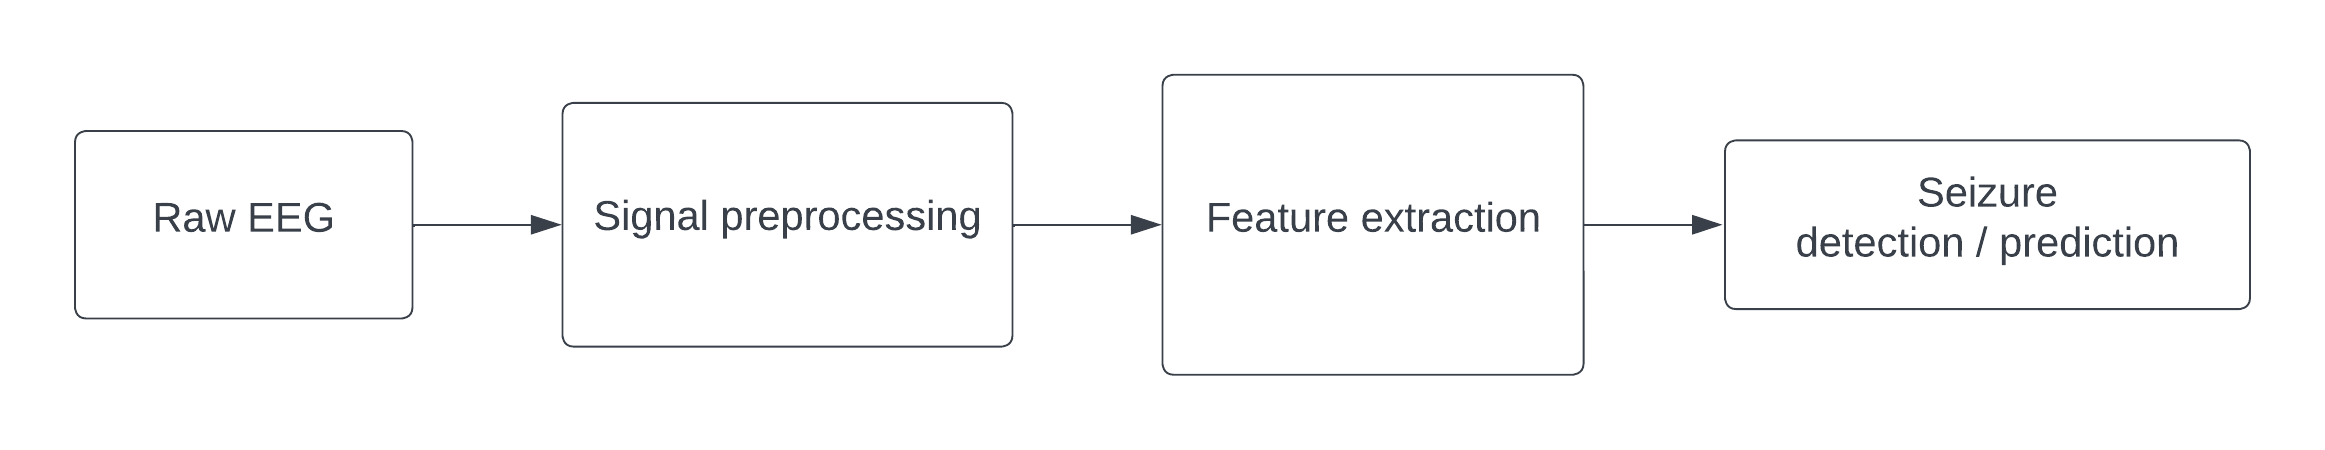
\includegraphics[width=1.0\textwidth]{images/State-of-art/traditional-feature-extraction-classification.png}
    \caption{Traditional feature extraction and classification methods combined}
    \label{fig:traditional-feature-extraction-classification}
\end{figure}

\subsection{Deep learning algorithms}
Deep learning algorithms are a type of \gls{AI} that are designed to recognize patterns and make decisions or predictions based on data inputs without the need for specialized feature extraction techniques. In recent years, deep learning algorithms have been implemented in a variety of applications, including in the field of healthcare. 

Deep learning algorithms, can address some limitations of traditional techniques, but also come with their disadvantages. 

One example is \gls{CNN}, consisting of feature extraction and classification combined, saving them time, and reducing computational complexity.

The main drawback which deep learning algorithms suffer from is the lack of big datasets to sufficiently train the implemented models. The problem is made worse by the fact that seizures are relatively rare, therefore the available datasets are fairly unbalanced. Furthermore, as explained previously, seizures patterns differ greatly between patients because of variability in their specific brain condition.

\section{Datasets}
To develop accurate early detection and prediction of epileptic activity using \gls{EEG} signals, several key elements are necessary: a reliable and reproducible artificial intelligence algorithm, high-quality data, and sufficient computing power \cite{handa_open_2021}. There are various types of \gls{EEG} recordings, including intracranial, scalp, and ambulatory, which can be recorded in video, image, or signal format depending on the intended use in hospitals. There is a significant demand for real-time biomedical multimedia tools for analyzing and recognizing patterns in this data.

There are various datasets of \gls{EEG} recordings that are used for the diagnosis of epilepsy, and these datasets may be freely available or privately held for various reasons such as ethical considerations.

The main freely available datasets are summarized in Table \ref{tab:free-datasets}. What follows is a more in depth description for each one of them.

\begin{table}[ht]
    \centering
    \resizebox{\columnwidth}{!}{
        \begin{tabular}{cccccccc}
        \hline
        Ref. & Type                                                             & Year & Size    & \begin{tabular}[c]{@{}c@{}}No. of \\ channels\end{tabular} & \begin{tabular}[c]{@{}c@{}}No. of \\ patients\end{tabular} & \begin{tabular}[c]{@{}c@{}}Sampling \\ frequency (Hz)\end{tabular} & EEG labels                                                                                                  \\ \hline
        \cite{andrzejak_indications_2001}                        & Adult                                                            & 2001 & 3.05 MB & 128                                                        & 5                                                          & 173.61                                                             & seizure states, healthy                                                                                     \\
        \cite{shoeb_application_2009}                       & Paediatric                                                       & 2010 & 40 GB   & 24-27                                                      & 24                                                         & 256                                                                & ictal, non-ictal                                                                                            \\
        \cite{andrzejak_nonrandomness_2012}                        & Adult                                                            & 2012 & 814 MB  & 64                                                         & 5                                                          & 512, 1024                                                                & focal, non-focal                                                                                            \\
        \cite{howbert_forecasting_2014}                        & \begin{tabular}[c]{@{}c@{}}Dog and \\ human\end{tabular}         & 2014 & 105 GB  & -                                                          & -                                                          & 256                                                                & \begin{tabular}[c]{@{}c@{}}normal, focal \\ and generalized\end{tabular}                                    \\
        \cite{obeid_temple_2016}                        & Adult                                                            & 2015 & 572 GB  & 20-31                                                      & 10874                                                      & \begin{tabular}[c]{@{}c@{}}250, 256, \\ 512\end{tabular}                                                      & different types                                                                                             \\
        \cite{swami_eeg_2016}                        & Adult                                                            & 2016 & 604 KB  & 57                                                         & 10                                                         & 200                                                                & \begin{tabular}[c]{@{}c@{}}Ictal, interi-ictal,\\ pre-ictal EEGs\end{tabular}                               \\
        \cite{stevenson_dataset_2018}                       & \begin{tabular}[c]{@{}c@{}}Paediatric \\ (neonates)\end{tabular} & 2018 & 4.3 GB  & 19                                                         & 79                                                         & 256                                                                & seizure onset                                                                                               \\
        \cite{panwar_single_2020}                       & Adult                                                            & 2020 & 20 MB   & -                                                          & 15                                                         & 173.61                                                             & seizure onset                                                                                               \\
        \cite{detti_paolo_siena_2020}                       & Adult                                                            & 2020 & 20 GB   & 29                                                         & 14                                                         & 512                                                                & \begin{tabular}[c]{@{}c@{}}seizure onset, \\ seizure type\end{tabular}                                      \\
        \cite{nasreddine_epileptic_2021}                       & Adult                                                            & 2021 & 3 GB    & 21                                                         & 6                                                          & 500                                                                & \begin{tabular}[c]{@{}c@{}}Complex partial, \\ electrographic\\ and video-detected \\ seizures\end{tabular} \\
        \cite{cserpan_dataset_2021}                        & \begin{tabular}[c]{@{}c@{}}Paediatric \\ and Adult\end{tabular}  & 2021 & 15 GB   & 52                                                         & 30                                                         & 2000 Hz                                                            & HFO markings                                                                                                \\ \hline
        \end{tabular}
    }
    \caption{Freely-available epilepsy datasets \cite{handa_open_2021}}
    \label{tab:free-datasets}
\end{table}

\subsubsection{Bonn EEG time series database}
This database was the first \gls{EEG} dataset to be publically available for research applications in this field \cite{andrzejak_indications_2001}. 

It contains 100 single channel \gls{EEG} recordings taken from a 128 channel acquisition system. The recordings are 23.6 seconds long and have a sampling rate of 173.61 Hz. The spectral bandwidth range is between 0.5 Hz and 85 Hz. The database includes \gls{EEG} recordings from healthy patients with their eyes closed and open, as well as from epileptic patients both during seizure-free periods and during epileptic seizures. The data is presented in ASCII code and has been filtered with a band pass filter with cut off frequencies of 0.53 Hz and 40 Hz. 

It is artifact-free and does not require pre-processing for the classification of healthy and unhealthy signals. The data was made available in 2001 and the extended version is now part of the EPILEPSIA project.

\subsubsection{\glsentrylong{CHB-MIT} database}
This dataset contains \gls{EEG} recordings from 23 pediatric patients with epilepsy and one adult, who were given anti-seizure medications \cite{shoeb_application_2009, shoeb_chb-mit_2010}. The recordings were taken over a continuous period of 952 hours, and about 200 seizures were recorded. The recordings were taken using 24-27 \gls{EEG} channels with a sampling frequency of 256 Hz. Each recording segment is one hour long, and there are a total of 9-42 \gls{EDF} files per patient. 

The dataset also includes vagal nerve stimulus signals and separate file names and montages for seizure and non-seizure episodes.

\subsubsection{Bern-Barcelona EEG database}
This multi-channel \gls{EEG} database includes \gls{EEG} recordings from five patients with epilepsy, who underwent surgery in an attempt to achieve seizure freedom \cite{andrzejak_nonrandomness_2012}. 

The data includes both focal and non-focal \gls{EEG} and was recorded using specialized electrodes at a sampling rate of either 512 or 1024 Hz, depending on the number of channels used in the \gls{EEG} system. Each file includes approximately 10240 samples over a 20 second time period.

\subsubsection{American Epilepsy Society Seizure Prediction Challenge database}
This database consists of intracranial \gls{EEG} segments recorded from dogs and humans with various characteristics such as sampling rate, duration of \gls{EEG} recordings, and number of electrodes \cite{howbert_forecasting_2014}. It was released as part of a Kaggle challenge hosted by the American Epilepsy Society in 2014 for the development of seizure forecasting systems, and it was used by 504 teams. 

The database includes different seizure segments, including ictal, pre-ictal, post-ictal, and inter-ictal, which are provided in MATLAB files. The database is approximately 105 GB in size and includes additional annotated \gls{EEG} data provided by the University of Pennsylvania and the Mayo Clinic.

\subsubsection{\glsentrylong{TUH-EEG} corpus}
The Temple University \gls{EEG} corpus is the largest collection of freely available \gls{EEG} data used for the diagnosis of epilepsy and different types of seizures \cite{obeid_temple_2016}. It includes data collected from 2000 to 2013 from around 10874 patients in various clinical settings. 

The community behind this corpus has also developed various tools and software products for the analysis and annotation of \gls{EEG}, \gls{EMG}, and \gls{ECG} data, including an \gls{EDF} browser that allows users to view \gls{EEG} recordings in video form. Within the corpus, there are several different datasets available, including the \gls{IBMFT}, the \gls{TUH-EEG} epilepsy corpus, seizure corpus, slowing corpus, and events corpus.

\subsubsection{Neurology and sleep center, New Delhi EEG dataset}
This \gls{EEG} database consists of data recorded from patients with epilepsy, and is divided into three categories: ictal, pre-ictal, and inter-ictal stages \cite{swami_eeg_2016}. It was recorded using a Grass Tele-factor Comet AS40 Amplification System with 57 channels, and has a sampling rate of 200 Hz and a spectral bandwidth range of 0.5 Hz to 70 Hz. Each file in the database has 1024 samples, and a subset of the database is publicly available.

\subsubsection{A dataset of neonatal EEG recordings with seizures annotations}
This database is a collection of multi-channel \gls{EEG} recordings of 79 newborn babies, 39 of whom experienced neonatal seizures in the \gls{NICU} at Helsinki University Hospital in Finland \cite{stevenson_dataset_2018}. The \gls{EEG} signals were recorded using the NicOne \gls{EEG} amplifier and a 19-channel cap, with a sampling rate of 256 Hz and stored in \gls{EDF} files. 

The data includes seizure annotations made by healthcare professionals for the purpose of seizure detection, and has been pre-processed using butterworth high-pass filtering.

\subsubsection{Single electrode EEG data of healthy and epileptic patients}
This dataset was created for the purpose of developing a predictive model for epilepsy diagnosis and has been publicly available since 2020. It was generated using similar acquisition and settings, such as sampling frequency, bandpass filtering, number of signals, and time duration, as the University of Bonn dataset \cite{panwar_automated_2019, panwar_single_2020}. 
However, it addresses some of the limitations of the University of Bonn dataset, such as using different \gls{EEG} recording methods (intracranial and scalp) for healthy and epileptic patients. All of the data in this dataset were collected exclusively using surface \gls{EEG} electrodes from 15 healthy and epileptic patients.

\subsubsection{Siena Scalp EEG Database}
The Siena Scalp EEG database includes \gls{EEG} recordings from 14 epileptic patients (9 males and 5 females), which were collected using specialized amplifiers and reusable electrodes \cite{detti_eeg_2020, detti_paolo_siena_2020}. The signals were recorded at a sampling rate of 512 Hz and stored in \gls{EDF} files. The data was collected at the University of Siena in Italy as part of a national interdisciplinary research project focused on seizure prediction, project PANACEE. 

The database includes 47 seizures from 128 hours of video \gls{EEG} recordings, and also includes the start and end times of seizures and the list of electrodes used during the recordings. The data includes three types of seizures: focal onset with and without impaired awareness, and focal to bilateral tonic-clonic seizures.

\subsubsection{Epileptic EEG Dataset}
This database contains long term \gls{EEG} data recorded from six patients with focal epilepsy who were being evaluated for possible epilepsy surgery \cite{nasreddine_epileptic_2021}. The data includes various stages of seizures, such as ictal, pre-ictal, inter-ictal, and onsets. The \gls{EEG} signals were recorded at a sampling rate of 500 Hz and stored in \gls{EDF} files. 

The data has been labeled and classified for use in training and testing for the detection of complex partial electrographic and videodetected seizures. The \gls{EEG} signals were also filtered with a bandpass range of 1-70 Hz, with 50 Hz removed.


\subsubsection{Dataset of EEG recordings of pediatric patients with epilepsy based on the 10-20 system}
The purpose of this dataset is to investigate the relationship between age and \glspl{HFO} in epileptic patients \cite{cserpan_dataset_2021}. The dataset consists of 3 hours of \gls{EEG} recordings from 30 patients, 15 children and 15 adults, with focal or generalized epilepsy. The recordings were made during sleep and have a sampling rate of 2000 Hz. The data is stored in \gls{EDF} files and includes sleep stage annotations.

\subsection{The dataset used: \glsentryshort{CHB-MIT}} \label{subsec:dataset-used}
I have chosen to use \gls{CHB-MIT} dataset for several reasons. Firstly, it was important for the dataset to be freely available for use in my research. This allowed me to easily access the data and incorporate it into my study without any financial barriers \cite{shoeb_application_2009, shoeb_chb-mit_2010}.

Secondly, the labels provided in the dataset needed to be suitable for my specific problem. In this case, I needed labels such as preictal, interictal or seizure, non-seizure to accurately analyze the data for my research. The availability of these labels in the dataset made it an ideal choice for my study.

Additionally, the dataset needed to contain sufficient data for deep learning training. This was crucial in order to ensure that the machine learning models used in my research would be able to accurately classify the \gls{EEG} signals.

Furthermore, the dataset needed to contain scalp \gls{EEG} recording for its potential practical applications rather than \gls{iEEG}, which is invasive and requires surgery.

Finally, it was important for the dataset to have been used in published works that are similar to mine in order to perform more accurate comparisons in my research. The use of a dataset with a proven track record in similar studies provided a strong foundation for my own work.

\subsubsection{Potential alternatives}
In considering alternative datasets for my research, the Siena Scalp EEG Database and the \gls{TUH-EEG} corpus were initially selected. Ultimately, the \gls{CHB-MIT} dataset was chosen for several reasons, first of which the size of the dataset: the Siena dataset, while containing useful data, was relatively small with only around 100 hours of \gls{EEG} recordings from 14 patients. On the other hand, the \gls{TUH-EEG} corpus was significantly larger with over 500 GB of data, but was unfortunately not available for use at the time of my research.

Finally, the choice of \gls{CHB-MIT} dataset was also justified by the fact that it had been used in published research that was similar to my own, allowing me to make more accurate comparisons. 

While it should be noted that the \gls{CHB-MIT} dataset is a pediatric database, the availability of other works using this dataset made it the best choice for my research.

\subsubsection{In depth description}
The \gls{CHB-MIT} dataset consists of \gls{EEG} recordings from 24 patients in total, with each case containing between 9 and 42 continuous \gls{EDF} files \cite{shoeb_chb-mit_2010}. The recordings were collected from 22 pediatric subjects, 5 of whom were male and 17 of whom were female and one adult (chb24). The case chb21 was obtained 1.5 years after case chb01, from the same female subject; the chb24 case was added to the collection in December 2010 and its age is unknown, aside for the fact of this patient being at least 18 years old. The ages of the pediatric subjects ranged from 1.5 to 22 years old.

The \gls{EDF} files contain dates that have been replaced with surrogate dates, but the time relationships between the files within each case have been preserved. Most of the files contain one hour of digitized \gls{EEG} signals, although some are shorter or longer. 

The \gls{EEG} signals were recorded using the International 10-20 system of electrode positions and were sampled at 256 samples per second with 16-bit resolution. Some of the recordings also include additional signals such as an \gls{ECG} or a \gls{VNS}. 

The collection includes a total of 664 \gls{EDF} files, 129 of which contain one or more seizures. There are a total of 198 seizures in the collection, 182 of which were in the original set of 23 cases. Information about the montage used for each recording and the elapsed time of each seizure is included in a summary text file. It should be noted that the montage used is subject to changes even within the very same recording.

It is proposed in this work to utilize only records that conform to a particular 21 electrodes montage of 23 channels from 24 subjects. 
Such montage is represented in Fig. \ref{fig:23-channels-montage}.
Each channels represent the voltage difference between the electrode potentials at the two ends of the arrows and is referred to as $X$-$Y$, where $X$ is the first electrode and $Y$ the second (i.e. F4-C3).

Records featuring variations in electrodes and montages have been excluded. 

These decisions resemble those in the reference works about to be presented.

Several details concerning the patients in the chosen dataset are presented in Table \ref{tab:chb-mit-content}.

\begin{figure}[ht]
    \centering
    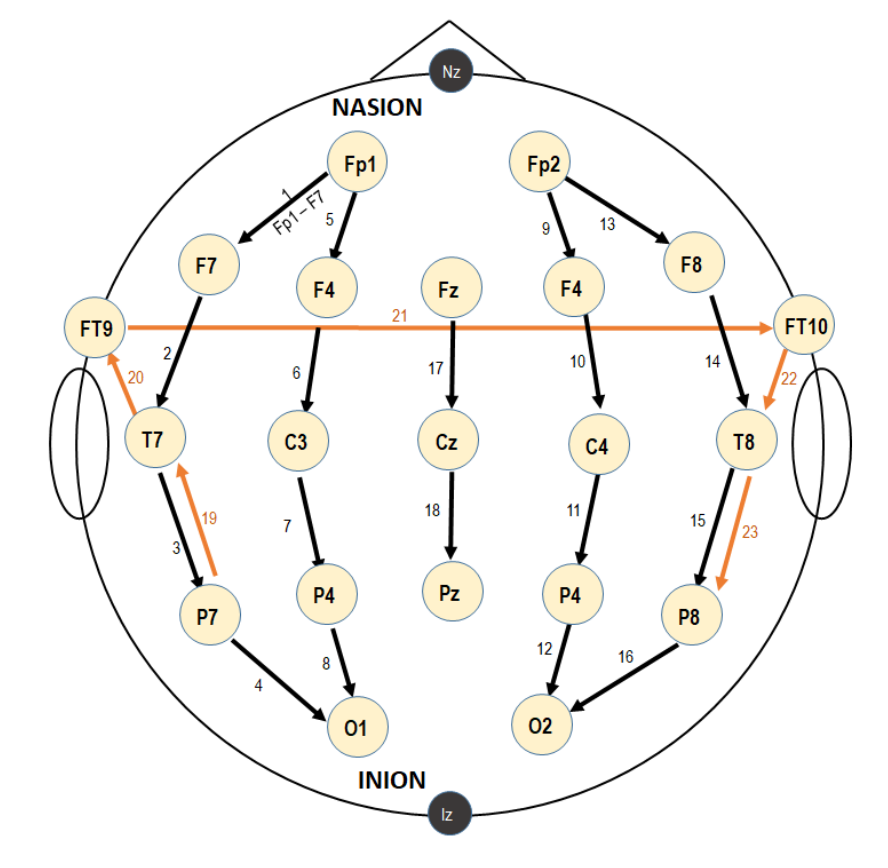
\includegraphics[width=0.75\textwidth]{images/State-of-art/23-channels-montage.png}
    \caption{21 electrodes montage of 23 channels used}
    \label{fig:23-channels-montage}
\end{figure}

\begin{table}[ht]
    \centering
    \resizebox{\columnwidth}{!}{
        \begin{tabular}{cccccc}
        \hline
        Patient & Gender-Age & Seizures & \begin{tabular}[c]{@{}c@{}}Total\\ seizure\\ duration (s)\end{tabular} & \begin{tabular}[c]{@{}c@{}}Total\\ recordings (h)\end{tabular} & \begin{tabular}[c]{@{}c@{}}Total\\ recordings (h)\\ only seizure records\end{tabular} \\ \hline
        chb01   & F-11       & 7        & 442                                                                    & 40.55                                                          & 6.65                                                                                  \\
        chb02   & M-11       & 3        & 172                                                                    & 35.27                                                          & 2.27                                                                                  \\
        chb03   & F-14       & 7        & 402                                                                    & 38.00                                                          & 7.00                                                                                  \\
        chb04   & M-22       & 4        & 378                                                                    & 156.07                                                         & 10.66                                                                                 \\
        chb05   & F-7        & 5        & 558                                                                    & 39.00                                                          & 5.00                                                                                  \\
        chb06   & F-1.5      & 10       & 153                                                                    & 66.74                                                          & 25.89                                                                                 \\
        chb07   & F-14.5     & 3        & 325                                                                    & 67.05                                                          & 9.04                                                                                  \\
        chb08   & M-3.5      & 5        & 919                                                                    & 20.01                                                          & 5.00                                                                                  \\
        chb09   & F-10       & 4        & 276                                                                    & 67.87                                                          & 9.58                                                                                  \\
        chb10   & M-3        & 7        & 447                                                                    & 50.02                                                          & 14.02                                                                                 \\
        chb11   & F-12       & 3        & 806                                                                    & 34.79                                                          & 2.79                                                                                  \\
        chb12   & F-2        & 27       & 989                                                                    & 20.69                                                          & 9.68                                                                                  \\
        chb13   & F-3        & 10       & 440                                                                    & 11.00                                                          & 7.00                                                                                  \\
        chb14   & F-9        & 8        & 169                                                                    & 26.00                                                          & 7.00                                                                                  \\
        chb15   & M-16       & 20       & 1992                                                                   & 39.01                                                          & 14.01                                                                                 \\
        chb16   & F-7        & 8        & 69                                                                     & 17.00                                                          & 5.00                                                                                  \\
        chb17   & F-12       & 3        & 293                                                                    & 20.01                                                          & 3.01                                                                                  \\
        chb18   & F-18       & 6        & 317                                                                    & 34.63                                                          & 5.63                                                                                  \\
        chb19   & F-19       & 3        & 236                                                                    & 28.93                                                          & 2.93                                                                                  \\
        chb20   & F-6        & 8        & 294                                                                    & 27.60                                                          & 5.57                                                                                  \\
        chb21   & F-13       & 4        & 199                                                                    & 32.83                                                          & 3.83                                                                                  \\
        chb22   & F-9        & 3        & 204                                                                    & 31.00                                                          & 3.00                                                                                  \\
        chb23   & F-6        & 7        & 424                                                                    & 26.56                                                          & 8.96                                                                                  \\
        chb24   & Adult      & 16       & 511                                                                    & 21.30                                                          & 12.00                                                                                 \\ \hline
        Total   &            & 181      & 11015                                                                  & 951.93                                                         & 185.51                                                                                \\ \hline
        \end{tabular}
    }
    \caption{\glsentrylong{CHB-MIT} dataset content overview in an epilepsy prediction perspective \cite{shoeb_chb-mit_2010}}
    \label{tab:chb-mit-content}
\end{table}

Records that include seizures are designated as seizure records, while the rest are referred to as non-seizure records. Ground truth is provided for seizure records in the form of expert-determined start and end points for the seizures. Fig. \ref{fig:chb-mit-recordings} illustrates the sequence of seizure and non-seizure records for one patient.

\begin{figure}[ht]
    \centering
    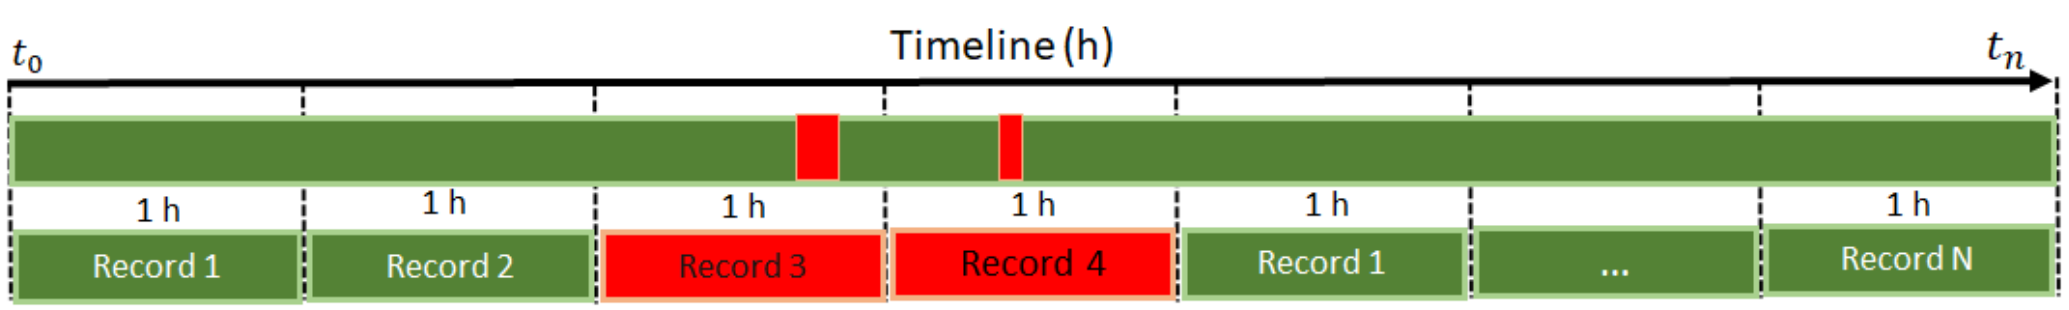
\includegraphics[width=1.0\textwidth]{images/State-of-art/chb-mit-recordings.png}
    \caption{Illustrative timeline for the patient chb01 which seizure segments red shaded. Analogously, record
files contain seizures are red shaded, otherwise are green shaded}
    \label{fig:chb-mit-recordings}
\end{figure}


\section{Reference works}
This thesis will use the results, frameworks, and techniques from three previous works on the \gls{CHB-MIT} dataset \cite{shoeb_chb-mit_2010} as references.

\begin{table}[ht]
    \centering
    \begin{tabular}{|c|c|c|} \hline  
        \glsentryshort{UNISI} & \glsentryshort{UAB} & \glsentryshort{UNISA} \\ \hline\hline
            patient specific               & patient generic        & \begin{tabular}[c]{@{}c@{}}patient generic\\ \&\\ patient specific\end{tabular} \\  \hline
            seizure prediction             & seizure detection      & seizure prediction \\  \hline
            traditional feature extraction & deep anomaly detection & deep CNN \\  \hline
        \end{tabular}
    \caption{Summarized comparison between reference works}
    \label{tab:summarized-comparison-reference-works} 
\end{table}


\subsubsection{Evaluation metrics} \label{subsub:evaluation-metrics}

The works that have been taken into consideration use the following metrics:

\begin{itemize}
    \item $pred\%$ is the percentage of test seizures correctly predicted. A seizure is considered correctly predicted if the first window whose output label is \textit{preictal} is located at most 300 seconds before the onset, if such is the parameter used as preictal duration as it is in the works presented in this thesis.
    \item $spec\%$ is the windows specificity, computed as
    
        \begin{equation}
            \frac{TN}{FP+TN}
        \end{equation}
        
    \item $\overline{t}_p$ is the average prediction time in seconds
    \item $t_p^m$ is the minimum prediction time in seconds
    \item $t_p^M$ is the maximum prediction time in seconds
\end{itemize}

$\overline{t}_p$, $t_p^m$ and $t_p^M$ only consider the first window labaled as preictal among the windows obtained from the seizure record.

Furthermore, other heuristic metrics have been introduced in this work to simplify the discussion around the quality of the results and the characteristics of expected ones. These metrics are

\begin{itemize}
    \item $\glsentryshort{IFP}$ (\glsentrylong{IFP}) is the average time between two false positive detections, in seconds, computed as
        \begin{equation}
            \frac{WD - WO}{1 - spec\%}
        \end{equation}
    \item $\overline{t}_w\%$ is the average worrying time percentage, computed as
        \begin{equation}
            \frac{\overline{t}_p}{IFP}
        \end{equation}    
    \item $t_w^m\%$ is the minimum worrying time percentage, computed as
        \begin{equation}
            \frac{t_p^m}{IFP}
        \end{equation}
    \item $t_w^M\%$ is the maximum worrying time percentage, computed as
        \begin{equation}
            \frac{t_p^M}{IFP}
        \end{equation}
\end{itemize}


\subsection{Patient Specific Seizures Prediction with Traditional Techniques} \label{subsec:refwork-siena}
This work was carried out by \gls{UNISI} \cite{detti_patient-specific_2019, detti_paolo_siena_2020} on data from \gls{CHB-MIT} dataset and Siena Scalp \gls{EEG} Database \cite{detti_eeg_2020, detti_paolo_siena_2020}, but only the experiments involving the former will be considered.

It presents a patient specific approach for the prediction of epileptic seizures using traditional monovariate and bivariate feature extraction techniques and a simple thresholding algorithm for classification, as shown in Fig. \ref{fig:siena-feature-extraction}.

\begin{figure}[ht]
    \centering
    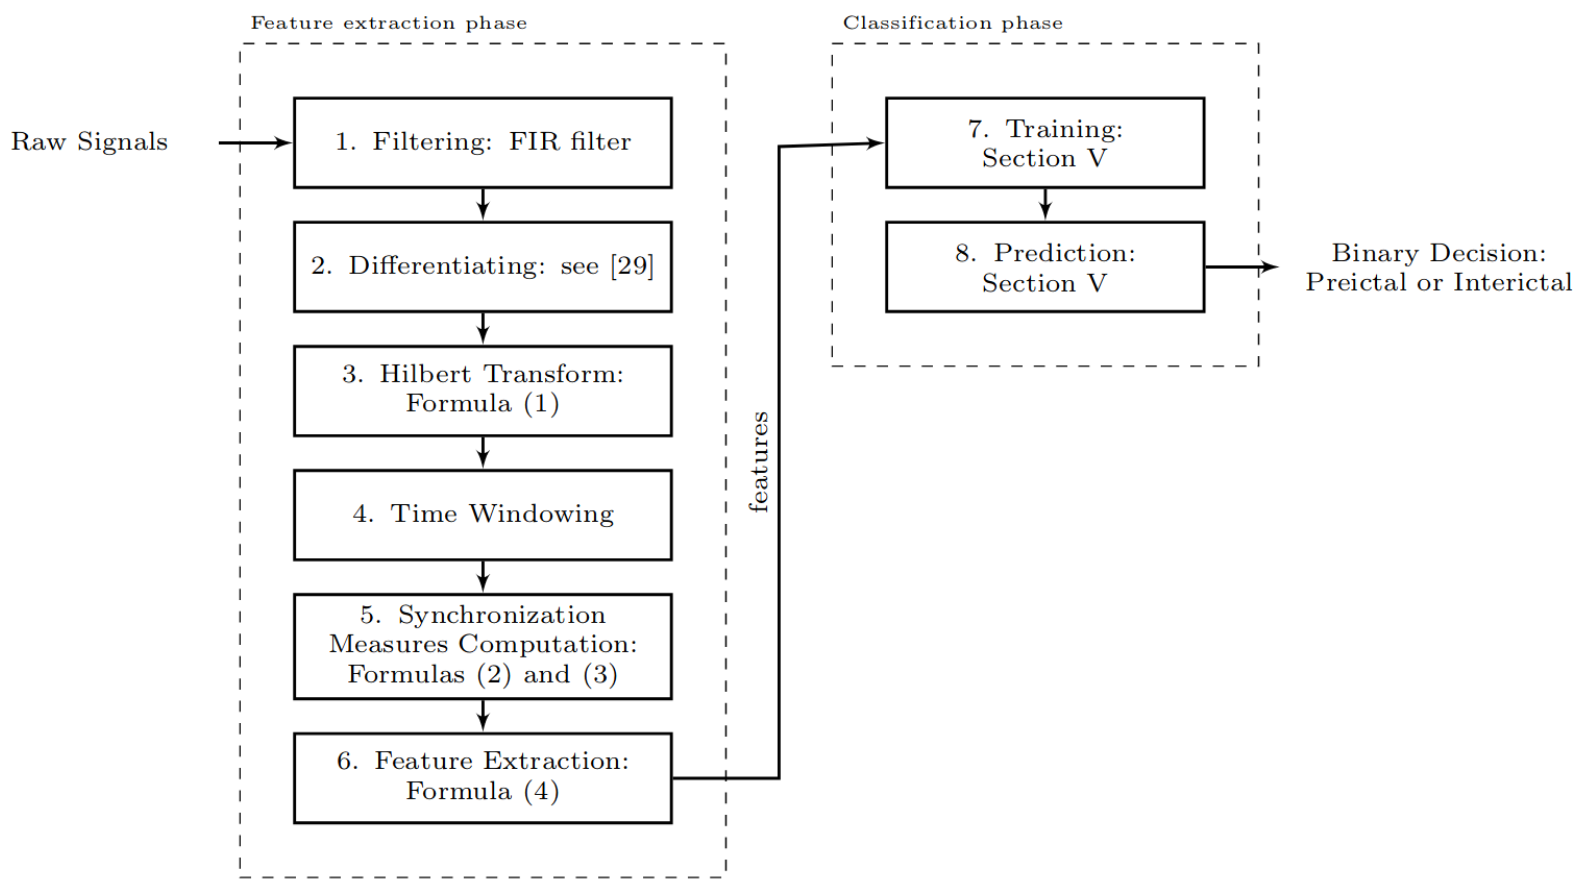
\includegraphics[width=1.0\textwidth]{images/State-of-art/siena-feature-extraction.png}
    \caption{Block diagram of the approach used in work from \gls{UNISI} \cite{detti_patient-specific_2019}}
    \label{fig:siena-feature-extraction}
\end{figure}


\subsubsection{Feature extraction}
The feature extraction from \gls{EEG} signals used in this work includes the following steps:
\begin{enumerate}
    \item The \gls{EEG} signals are filtered using a pass-band \gls{FIR} filter with band [8-13] \unit{Hz}.
    \item The time-derivative of the signals is computed to make the noise nearly flat and sharpen the regions where seizures occur.
    \item The analytical signals and their phases are extracted using the Hilbert transform.
    \item The signals are segmented into consecutive overlapping time windows. 
    Specifically, \gls{WD} is 6 seconds and \gls{WO} is 1 second.
    \item Synchronization measures \gls{PLI} and \gls{WPLI} are computed for each pair of signals and each time window.
        \begin{itemize}
            \item \gls{PLI} is based on the idea of discarding the phase differences that center around 0 (mod $\pi$). This allows to study short-term changes of increasing and decreasing synchronization.
            \item In \gls{WPLI}, each phase difference is weighted according to the magnitude of the lag, so that phase differences around zero only marginally contribute to the calculation of such metric.
        \end{itemize}
    \item Features are extracted from the synchronization measures using a graph model and a moving average procedure.
\end{enumerate}

\subsubsection{Classification}
The classification phase includes a training and a prediction step. 
\begin{enumerate}
    \setcounter{enumi}{6}
    \item The training step uses labeled data to train the classifier and may include a feature selection step to select the most promising features.
    \item The prediction step uses the trained classifier to assign a label (preictal or interictal) to new unlabeled data, which is the output of the whole process.
\end{enumerate}

\subsubsection{Experimental setup} \label{subsub:refwork-siena-exp}
Each patient's dataset is composed of several instances, each typically lasting about 1 hour. Some of these instances contain seizures, while others do not. In order to prepare the data for the prediction task, each seizure instance (which is usually 1 hour long) is divided into smaller instances, each containing a single seizure. 

Only the recordings (instances) with the same \gls{EEG} montage and number of EEG channels for each patient were considered.

The following steps were taken to prepare the data:
\begin{itemize}
    \item Discarding the ictal periods
    \item Discarding a postictal period of 1000 seconds.
    \item Removing seizure instances with a preictal period smaller than 300 seconds.
    \item Removing seizure instances where the period of time between the end of the preceding seizure and the beginning of the current seizure is smaller than 1300 seconds.
\end{itemize}

In the classification phase, a cross-validation approach is used for each patient to assess the quality of the prediction model.
For each patient, $q$ rounds of cross-validation are performed, with the additional condition that each seizure instance is selected for testing in at least one of the $q$ rounds. Denoted as $m_s$ the number of seizure instances of a patient, the parameter $q$ is set to $5$ for patients with $m_s > 4$ and to $m_s$ when $m_s = 3$.

For this reason some of the patients were discarded due to having too few seizure instances which don't allow a reasonable definition of training and testing sets for cross-validation.

The training method is \textit{patient specific}, which means that $N$ classifiers were trained, where $N$ is the number of patients considered. Each classifier was trained and tested only with the data associated with its specific patient.

\subsubsection{Claimed results} \label{subsub:refwork-siena-results}
Following there are two tables of results claimed by the authors.

In Table \ref{tab:siena-performance-seizure-sequence} results are reported that are directly associated with the possibility of a direct application of this classifier to a patient.
With an average $pred\%$ of 100\% it looks like the classifier should be able to detect every incoming seizure, but there are two important considerations to be made:
\begin{itemize}
    \item the average $spec\%$ is 95.97\%, which, when put in perspective with its \gls{WD} of 6 seconds and 1 second of \gls{WO}, gives an \gls{IFP} of about 124 seconds.
    \item the average $\overline{t}_p$ is about 79 seconds, which, when combined with the \gls{IFP} calculated above, gives a $\overline{t}_w\%$ of 64\%
    \item arguably $t_w^M\%$ is more interesting than $\overline{t}_w\%$, but in this case exceeds 100\%, reaching more accurately about 122\%.
    \item the average $t_p^m$ is about 10 seconds, but is 0 for many patients.
\end{itemize}

\begin{table}[ht]
    \centering
    \begin{tabular}{c|rrrrr}
    Pat.  & $pred\%$ & $spec\%$ & $\overline{t}_p$   & $t_p^m$  & $t_p^M$   \\ \hline
    chb01 & 100    & 98.73  & 29.4   & 0    & 122   \\
    chb03 & 100    & 99.53  & 47.13  & 14   & 158   \\
    chb04 & 100    & 97.41  & 42.1   & 0    & 115   \\
    chb05 & 100    & 100    & 66.7   & 21   & 143   \\
    chb06 & 100    & 91.74  & 198.48 & 9    & 293   \\
    chb07 & 100    & 99.94  & 29.33  & 0    & 49    \\
    chb08 & 100    & 99.34  & 51.2   & 0    & 210   \\
    chb09 & 100    & 99.29  & 12.3   & 0    & 35    \\
    chb10 & 100    & 100    & 39     & 19   & 70    \\
    chb12 & 100    & 71.41  & 243.95 & 22   & 292   \\
    chb13 & 100    & 83.49  & 221.67 & 47   & 291   \\
    chb14 & 100    & 95.1   & 42.35  & 0    & 113   \\
    chb15 & 100    & 93.77  & 178.3  & 8    & 295   \\
    chb16 & 100    & 97.9   & 102.7  & 12   & 218   \\
    chb17 & 100    & 98.66  & 76.67  & 19   & 175   \\
    chb18 & 100    & 99.91  & 38.1   & 14   & 49    \\
    chb20 & 100    & 95.84  & 28.6   & 0    & 82    \\
    chb21 & 100    & 99.35  & 52.3   & 4    & 128   \\
    chb22 & 100    & 100    & 17     & 1    & 32    \\
    chb23 & 100    & 98.04  & 60.07  & 9    & 142   \\ \hline
    Av.   & 100    & 95.97  & 78.87  & 9.95 & 150.6 \\ \hline
    \end{tabular}
    \caption{Seizure instance-wise performance of the traditional classification algorithm on \glsentrylong{CHB-MIT} dataset \cite{detti_patient-specific_2019}}
    \label{tab:siena-performance-seizure-sequence} 
\end{table}

Please note that this is one of the most recent and performing works in the field of epileptic seizure prediction but is still objectively unusable to improve the everyday life of a patient suffering from epilepsy.

\subsection[Patient Generic Seizures Detection with Unsupervised\\Anomaly Detection]{Patient Generic Seizures Detection with Unsupervised Anomaly Detection} \label{subsec:refwork-uab}
This work was carried out by a student of \gls{UAB} as a master thesis project.

The reason why this study has been chosen as reference is the complete lack of anomaly detection techniques in the field of epileptic seizure prediction and detection in scientific literature.

It presents a patient generic approach for the \textit{detection} (as opposed to \textit{prediction}) of epileptic seizures using almost raw \gls{EEG} data and an autoencoder based on \gls{LSTM} to carry out unsupervised anomaly detection.
\subsubsection{Feature extraction} \label{subsub:refwork-uab-featext}
The feature extraction from \gls{EEG} signals used in this work consists in the following steps:

\begin{enumerate}
    \item The signals are undersampled from the original 256 Hz of the \gls{CHB-MIT} to 128 Hz
    \item The 21 channels are combined in a single channel which contains, for each instant, the average value in the original ones
    \item The signals are segmented into consecutive time windows, with \gls{WD} of 2 seconds and no overlap.
\end{enumerate}

\subsubsection{The model}
The model chosen in this work is an \gls{LSTM}-based autoencoder with 4 \gls{LSTM} layers and 1 \gls{MLP} layer, as shown in Fig. \ref{fig:lstm-autoencoder-architecture}.

The model is trained to minimize reconstruction errors of the data in the training set, where the error is calculated as \gls{MSE} between the input and the output sequences.

\begin{figure}[ht]
    \centering
    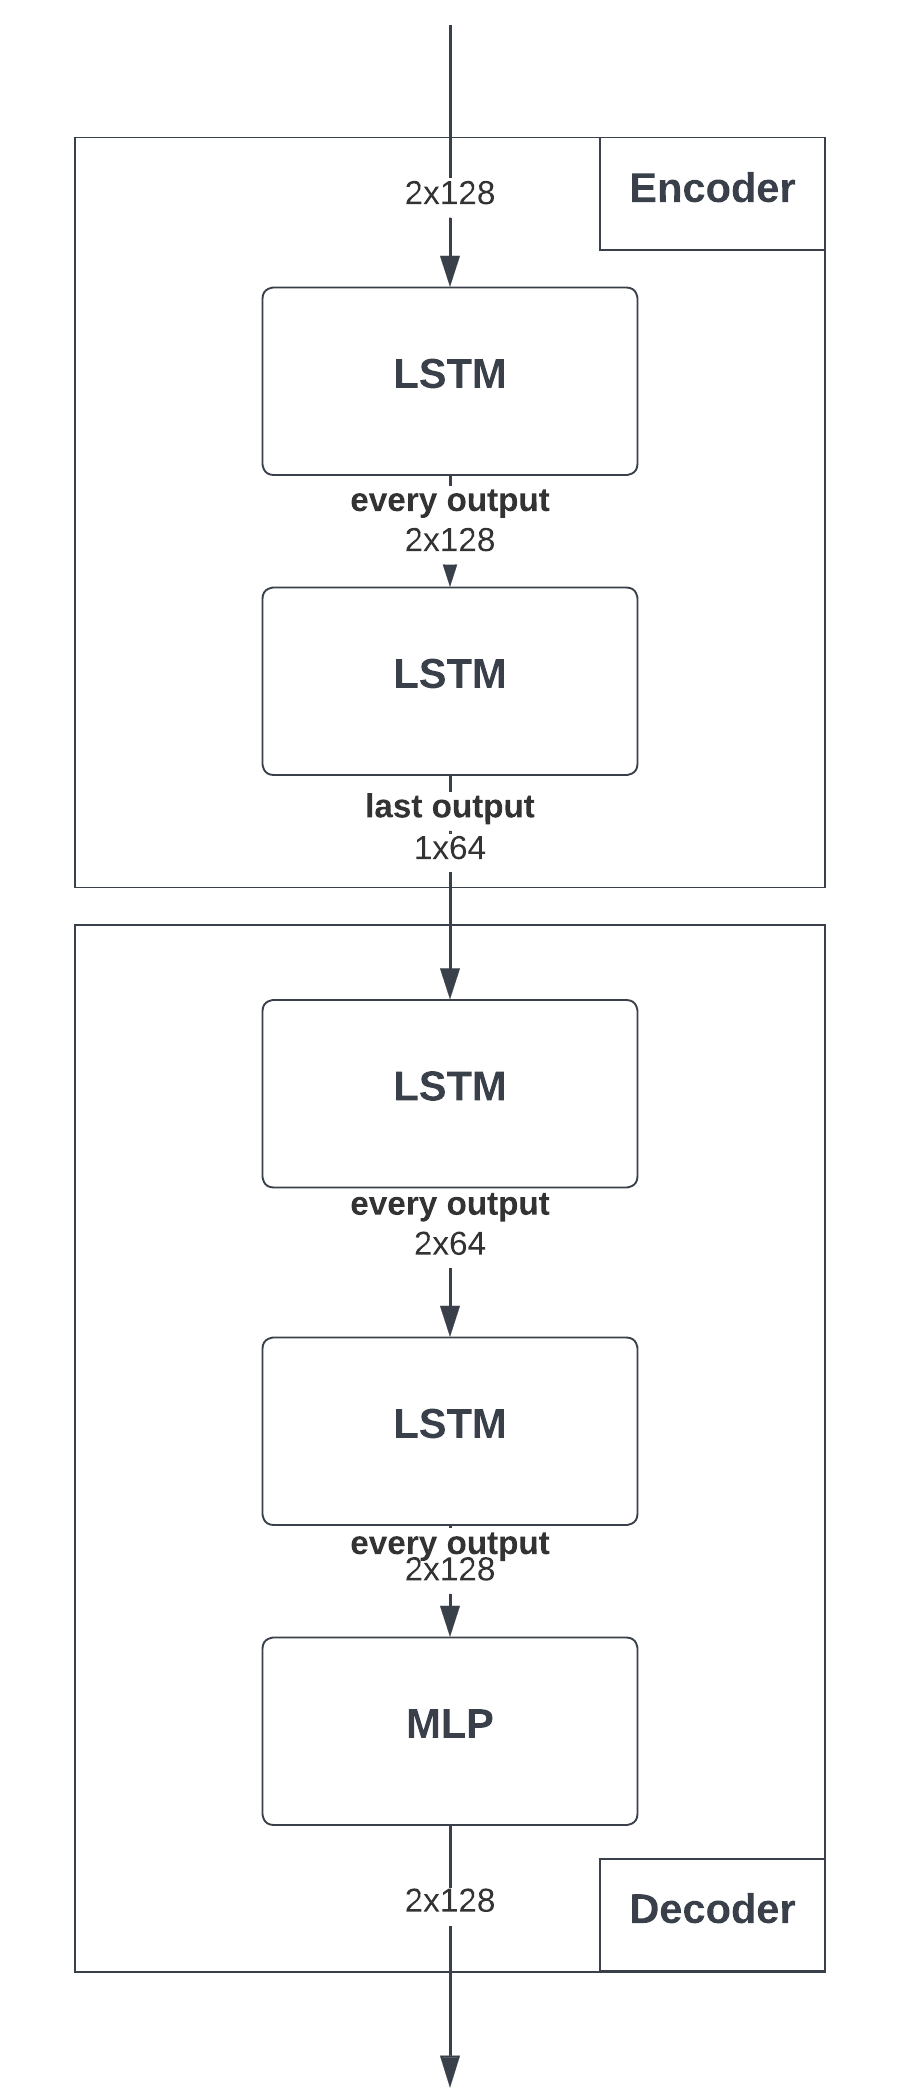
\includegraphics{images/State-of-art/lstm-autoencoder.png}
    \caption{Block diagram of the model used in work from \gls{UAB}}
    \label{fig:lstm-autoencoder-architecture}
\end{figure}

The total number of parameters is about 330 thousands. A summary of the network is shown in Fig. \ref{fig:lstm-summary}.

\begin{figure}[ht]
    \centering
    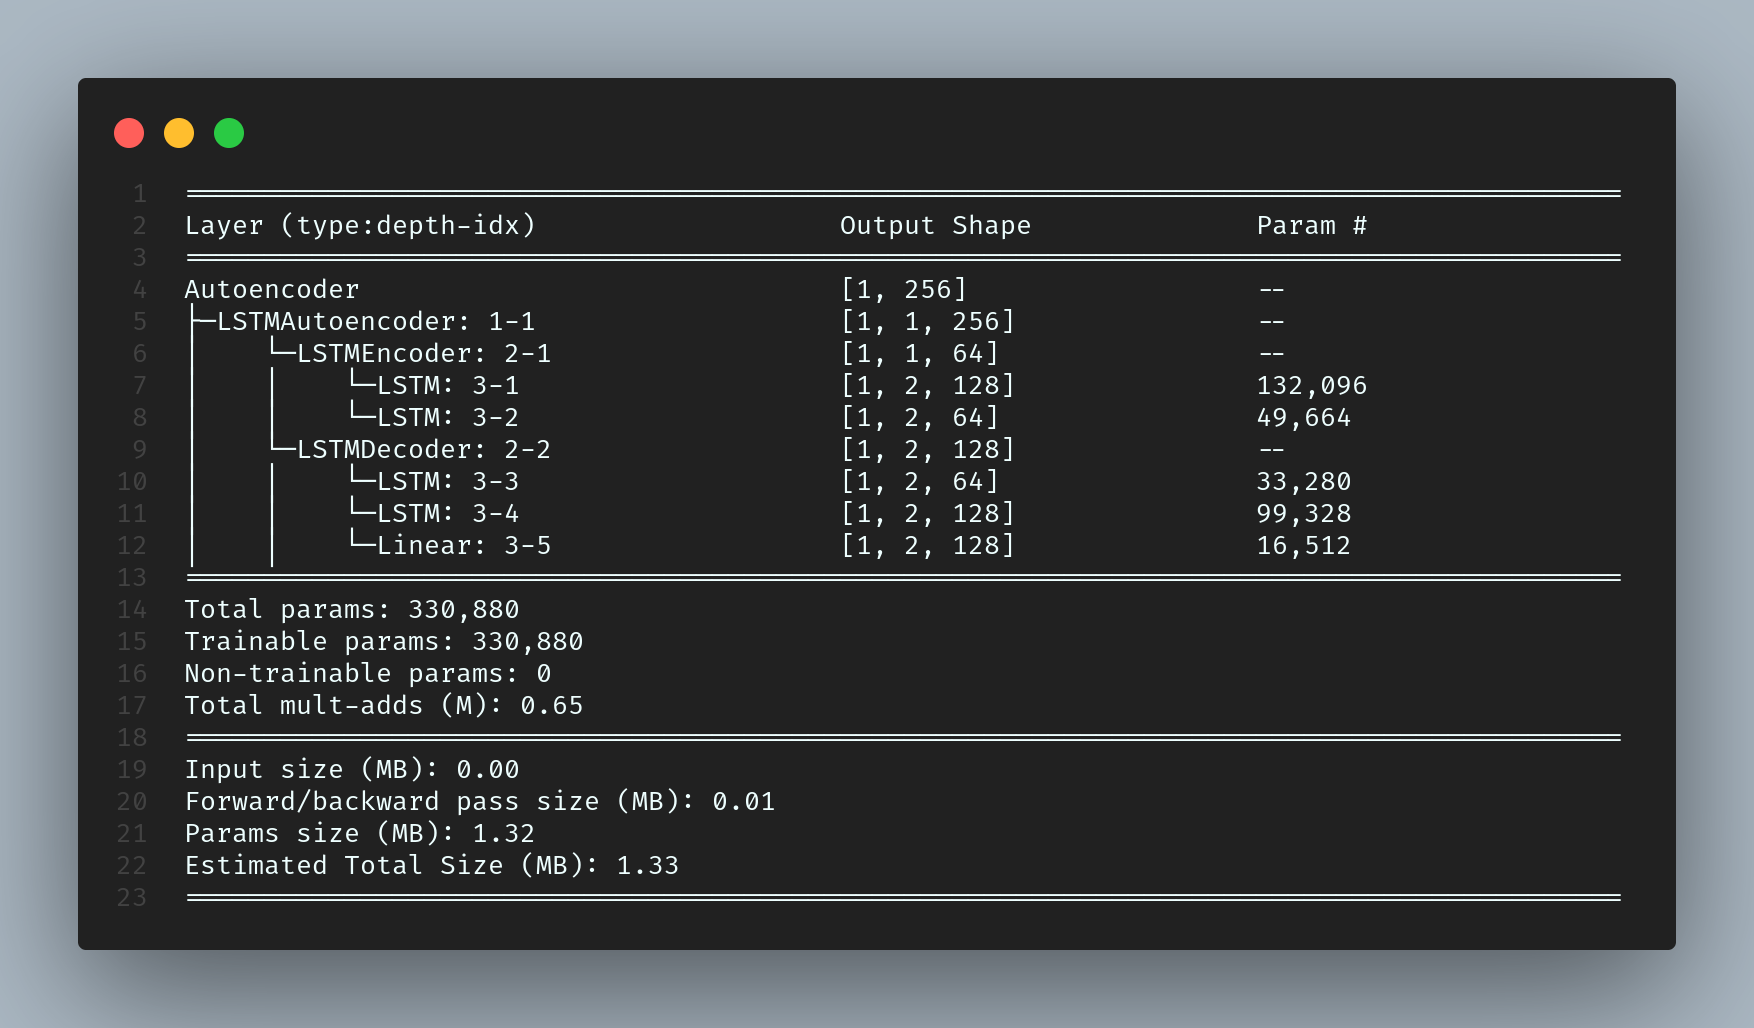
\includegraphics[width=1.0\textwidth]{images/State-of-art/lstm-summary.png}
    \caption{Summary of the LSTM autoencoder architecture, along with number of parameters. Produced using torchinfo \cite{yep_torchinfo_2020}}
    \label{fig:lstm-summary}
\end{figure}

\subsubsection{Experimental setup} \label{subsub:refwork-uab-exp}
This work follows the unsupervised anomaly detection paradigm, meaning that during the training phase only the normal instances will be submitted to the network.

The data preparation is the same as described in section \ref{subsub:refwork-siena-exp}.

Given that the model was only trained using normal instances, it was not necessary to discard those patient that had too few seizure instances, unlike the previous work.

The training method is \textit{patient generic} which means that only 1 classifier was trained using normal instances from all patients. The remaining normal instances and every seizure instances not discarded during the data preparation phase was included in the test set.

As previously mentioned, the neural network was trained to maximize quality of reconstruction, with the idea that records containing anomalies would be harder to reconstruct during the test phase. For this reason a threshold was found with the aim of getting the best possible separation between normal and anomalous samples. If the \gls{MSE} between the input and the output records is below the threshold, then the record is labeled as interictal, otherwise is labeled as preictal.

Such threshold is obtained on the training set applying the Otsu's method. Although it is not a suitable application for this algorithm, since it would normally require two classes, it achieved the desired result.

\subsubsection{Claimed results}
Following there are the claimed results for this work that I have also been able to reproduce.

As mentioned above, the training method was patient generic, therefore only average results were provided by the authors, as shown in Table \ref{tab:lstm-autoencoder-performance-spagnolo}.

\begin{table}[ht]
    \centering
    \begin{tabular}{c|c}
                  & percentage \\ \hline
        accuracy  & 86.5       \\
        precision & 87         \\
        recall    & 86         \\
        f1-score  & 86         \\ \hline
    \end{tabular}
    \caption{Windows-wise performance of the LSTM autoencoder \glsentrylong{CHB-MIT} dataset}
    \label{tab:lstm-autoencoder-performance-spagnolo} 
\end{table}


\subsection{Patient Specific and Patient Generic Seizures Predictions with CNN} \label{subsec:refwork-unisa}
Finally, this work was presented in a master thesis from \gls{UNISA} and developed in the same period of time as of the present study.

Such work follows both a patient specific and a patient generic approach, evaluate performance of supervised deep learning on a deep \gls{CNN} designed and optimized from scratch, reaching state-of-art performance.

It shares some preliminary operations with the study from \gls{UNISI} while eventually applying spectrogram transformations and treating them as images during the classification phase.



\subsubsection{Feature extraction} \label{subsub:refwork-unisa-featext}
The feature extraction from \gls{EEG} signals used in this work shares the first two steps with the work from \ref{subsec:refwork-siena}:
\begin{enumerate}
    \item The \gls{EEG} signals are filtered using a pass-band \gls{FIR} filter with band [8-13] \unit{Hz}.
    \item The time-derivative of the signals is computed to make the noise nearly flat and sharpen the regions where seizures occur.
\end{enumerate}

The next steps are instead unique to this works. This is, in fact, the point where the current study diverges from the normal state-of-art process:
\begin{enumerate}
    \setcounter{enumi}{2}
    \item A spectrogram is computed from the time-derivative of the \gls{EEG} signals using consecutive Fourier transforms of width 256 and no overlap.
    \item Discard the values outside of the first 40 Hz.
    \item Convert the values from magnitude to decibel.
\end{enumerate}

\subsubsection{The model}
The model is a \gls{CNN} network with multiple layers, ending with a dense classifier, as shown in Fig. \ref{fig:cnn-unisa-architecture}.

The network architecture includes 8 layers of 2D convolution using the \gls{ReLU} activation function, as well as 8 layers of batch normalization. Dimensionality reduction is achieved through the use of two max pooling layers. Additionally, there are 5 dropout layers with a drop rate of 0.1. 

The first half of the networks ends with a flattening layer, thus functioning effectively as a Feature Extractor. This neat functional distinction between the two halves in the network is of fundamental importance in the following study.

The seconds half of the network, which can functionally be considered as an \gls{MLP} classifier, is made of four dense layers. The first three layers use the \gls{ReLU} activation function. 

The last layer, or the output layer, however, utilizes a sigmoid activation function to map the output values in the interval between 0 and 1.

\begin{figure}[ht]
    \centering
    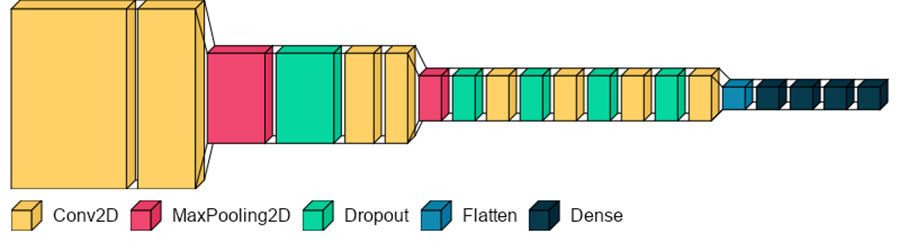
\includegraphics[width=1.0\textwidth]{images/State-of-art/cnn-unisa-architecture.png}
    \caption{Block representation of the CNN architecture used in work from \gls{UNISA}}
    \label{fig:cnn-unisa-architecture}
\end{figure}

The total number of parameters is about 15 million. A summary of the network is shown in Fig. \ref{fig:cnn-unisa-summary}.

\begin{figure}[ht]
    \centering
    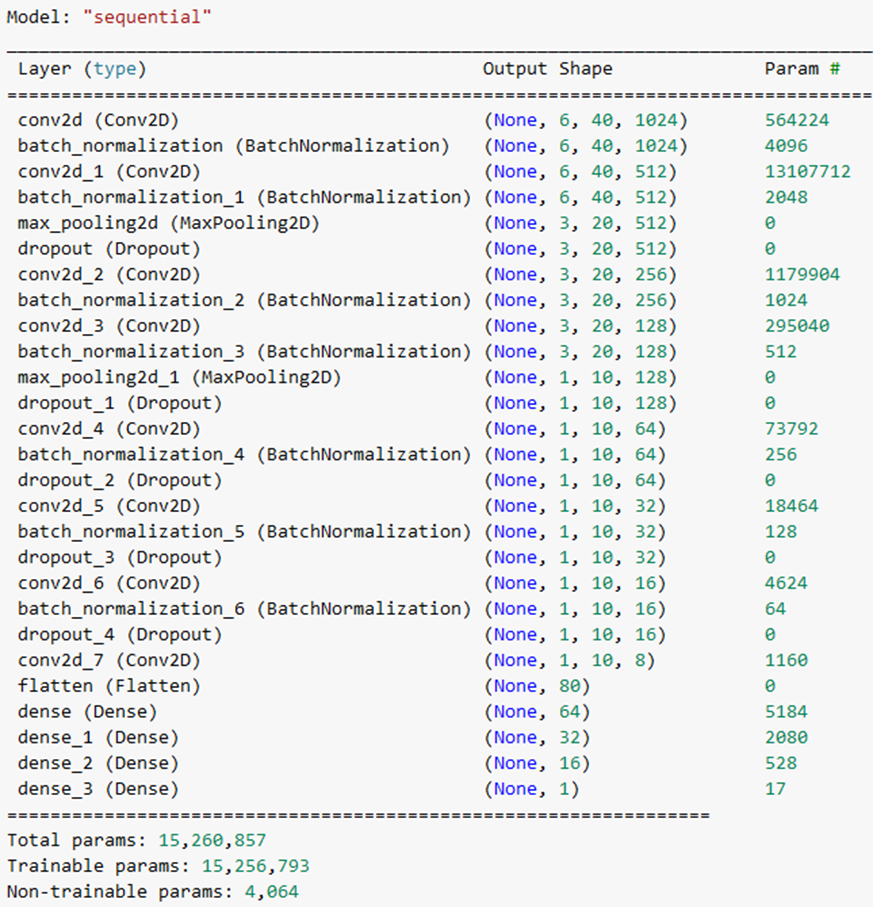
\includegraphics[width=1.0\textwidth]{images/State-of-art/cnn-unisa-summary.png}
    \caption{Summary of the CNN architecture, along with number of parameters, used in work from \gls{UNISA}}
    \label{fig:cnn-unisa-summary}
\end{figure}

\subsubsection{Experimental setup}
The experimental setup is exactly the same of that described in section \ref{subsub:refwork-siena-exp}.

There is a valuable addition, which is the adoption of a particular type of patient generic approach: differently from the experimental setup described in section \ref{subsub:refwork-uab-exp}, $N$ networks were trained, where $N$ is the number of patients considered. For each patient, its associated network was trained on the aggregated data from every other patient and tested on the data from the current patient, effectively performing a leave-one-patient-out validation.

In actuality, more experiments have been conducted in the work that is currently being described, that differ in preictal time and dataset used, but they are not important for the purposes of this thesis and therefore have been omitted.

\subsubsection{Claimed results}
What follows are the claimed results for the two experiments discussed in the previous section, which are patient specific and patient generic on \gls{CHB-MIT} dataset with a preictal time of 300 seconds.

In the patient specific results, some patients are missing for the same reason discussed in \ref{subsub:refwork-siena-exp}, i.e. insufficient seizure instances to allow the creation of meaningful training, validation and test sets.


\begin{table}[ht]
    \centering
    \begin{tabular}{c|rrrrr}
    Pat.  & $pred\%$ & $spec\%$ & $\overline{t}_p$   & $t_p^m$  & $t_p^M$   \\ \hline
    chb01 & 100    & 95.05  & 292.0  & 291    & 294    \\
    chb03 & 100    & 95.33  & 278.4  & 256    & 294    \\
    chb04 & 100    & 99.75  & 236.2  & 220    & 253    \\
    chb05 & 100    & 97.71  & 293.5  & 293    & 294    \\
    chb06 & 100    & 98.80  & 285.4  & 282    & 294    \\
    chb07 & 100    & 98.85  & 289.3  & 287    & 290    \\
    chb08 & 100    & 97.43  & 259.5  & 226    & 291    \\
    chb09 & 100    & 99.79  & 263.1 & 240    & 284    \\
    chb10 & 100    & 99.36  & 200.5  & 106    & 293    \\
    chb12 & 100    & 98.39  & 285.2  & 267    & 294    \\
    chb13 & 100    & 98.97  & 267.4  & 199    & 290    \\
    chb14 & 100    & 96.24  & 293.5  & 291    & 294    \\
    chb15 & 100    & 99.24  & 184.7  & 40     & 293    \\
    chb16 & 100    & 99.10  & 159.3  & 50     & 230    \\
    chb17 & 100    & 97.20  & 292.0  & 290    & 294    \\
    chb18 & 100    & 99.94  & 254.1  & 224    & 291    \\
    chb20 & 100    & 99.50  & 179.2  & 44     & 294    \\
    chb21 & 100    & 96.60  & 259.4  & 242    & 293    \\
    chb22 & 100    & 99.29  & 271.2  & 254    & 294    \\
    chb23 & 100    & 92.90  & 256.3  & 190    & 294    \\ \hline
    Av.   & 100    & 97.97  & 247.03 & 211.10 & 287.05 \\ \hline
    \end{tabular}
    \caption{Patient specific performance of the \gls{CNN} model on \glsentrylong{CHB-MIT} dataset}
    \label{tab:cnn-results-specific} 
\end{table}

In this case the reported results where almost on par with those shown in Section \ref{subsub:refwork-siena-results}: this time the average $pred\%$ also is 100\%, indicating that every incoming seizure should be successfully detected, but subtle differences are present:
\begin{itemize}
    \item the average $spec\%$ is 97.97\%, which, when put in perspective with its \gls{WD} of 6 seconds and 5 second of \gls{WO}, gives an \gls{IFP} of about 49 seconds. In the original work only the \gls{WD} was considered to compute the \gls{IFP}; even tho this measure gives a much more generous result of 296 seconds, it is unclear if with a different overlap the achieved prediction accuracy would still be 100\%.
    For comparison purposes an \gls{IFP} of 296 will be considered despite such uncertainty.
    \item the average $\overline{t}_p$ is about 247 seconds, which, when combined with the \gls{IFP} calculated above, gives a $\overline{t}_w\%$ of 84\%
    \item In this case the $t_w^M\%$ does not exceed 100\%, stopping at about 97\%.
    \item the average $t_p^m$ is about 211, which is much higher than the one presented in section \ref{subsub:refwork-siena-results}, with minimums around the 40 seconds mark.
\end{itemize}

In the patient generic case the same patients were also omitted, despite the aggregated data from every other patient was sufficient for creating suitable training and validation sets. In this case the aim of the authors of this work was to be able to compare the results to the work from section \ref{subsub:refwork-siena-exp}, which itself discarded the very same patients from the study.

\begin{table}[ht]
    \centering
    \begin{tabular}{c|rrrrr}
    Pat.  & $pred\%$ & $spec\%$ & $\overline{t}_p$   & $t_p^m$  & $t_p^M$   \\ \hline
    chb01 & 85.7   & 99.57  & 150.3  & 32    & 299   \\
    chb03 & 100.0  & 81.06  & 174.3  & 28    & 294   \\
    chb04 & 100.0  & 92.27  & 196.4  & 143   & 294   \\
    chb05 & 100.0  & 99.66  & 178.2  & 37    & 292   \\
    chb06 & 100.0  & 96.87  & 248.7  & 179   & 292   \\
    chb07 & 100.0  & 97.51  & 254.5  & 193   & 294   \\
    chb08 & 100.0  & 83.17  & 268.7  & 247   & 294   \\
    chb09 & 50.0   & 99.00  & 127.3  & 41    & 199   \\
    chb10 & 14.2   & 99.70  & 102.5  & 38    & 152   \\
    chb12 & 55.5   & 98.15  & 240.0  & 220   & 260   \\
    chb13 & 85.7   & 95.80  & 248.2  & 188   & 290   \\
    chb14 & 75.0   & 95.72  & 259.3  & 211   & 293   \\
    chb15 & 46.15  & 95.04  & 210.1  & 106   & 280   \\
    chb16 & 75.0   & 91.86  & 203.8  & 121   & 259   \\
    chb17 & 100.0  & 78.55  & 204.9  & 145   & 263   \\
    chb18 & 100.0  & 66.21  & 291.6  & 286   & 294   \\
    chb20 & 100.0  & 92.76  & 186.9  & 70    & 287   \\
    chb21 & 100.0  & 79.80  & 276.4  & 260   & 294   \\
    chb22 & 100.0  & 70.90  & 288.8  & 278   & 293   \\
    chb23 & 66.6   & 98.30  & 198.4  & 109   & 253   \\ \hline
    Av.   & 82.69  & 90.59  & 215.46 & 146.6 & 273.8 \\ \hline
    \end{tabular}
    \caption{Patient generic performance of the \gls{CNN} model on \glsentrylong{CHB-MIT} dataset}
    \label{tab:cnn-results-generic} 
\end{table}

In this case the reported results where considerably worse than the patient specific ones for this work, let alone those shown in Section \ref{subsub:refwork-siena-results}.

The average $pred\%$ is about 83\%, indicating that \textit{not} every incoming seizure should be successfully detected.
\begin{itemize}
    \item the average $spec\%$ is 90.59\%, is associated to an \gls{IFP} of about 64 seconds.
    \item the average $\overline{t}_p$ is about 215 seconds, associated with an $\overline{t}_w\%$ of 336\%
    \item the average $t_w^M\%$ is 428\%.
    \item the average $t_p^m$ is about 147, with minimums even below the 30 seconds mark.
\end{itemize}

Please note that the experiments were also successfully reproduced, obtaining the same results previously shown.


\section{Identification of possible advancements concerning the state-of-art}
Epileptic seizure prediction is a very important and unexplored subject in scientific literature. Only recently were deep learning techniques applied to try and solve the simpler task of epileptic seizure detection, achieving promising results.

Researches regarding epileptic seizure prediction remain extremely limited nonetheless but improvements in this field would mean getting close to a better and less worrying life for millions of people.

Although many studies for deep anomaly detection were carried out in the latest years, there are many possible applications that remain unexplored. Such is the case for the epileptic seizures prediction field.